\documentclass{article}

\usepackage{graphicx}
\usepackage{listings}

%http://tex.stackexchange.com/questions/140567/drawing-karnaughs-maps-in-latex
\usepackage{tikz}
\usetikzlibrary{matrix,calc}
%internal group
%#1 - Optional. Space between node and grouping line. Default=0
%#2 - top left node
%#3 - bottom right node
%#4 - filling color
\newcommand{\implicant}[4][0]{
	\draw[rounded corners=3pt, fill=#4, opacity=0.3] ($(#2.north west)+(135:#1)$) rectangle ($(#3.south east)+(-45:#1)$);
}

%Empty Karnaugh map 4x4
\newenvironment{Karnaugh}%
{
\begin{tikzpicture}[baseline=(current bounding box.north),scale=0.8]
\draw (0,0) grid (4,4);
\draw (0,4) -- node [pos=0.7,above right,anchor=south west] {ab} node [pos=0.7,below left,anchor=north east] {cd} ++(135:1);
%
\matrix (mapa) [matrix of nodes,
		column sep={0.8cm,between origins},
		row sep={0.8cm,between origins},
		every node/.style={minimum size=0.3mm},
		anchor=2.center,
		ampersand replacement=\&] at (0.5,0.5)
{
					   \& |(c00)| 00         \& |(c01)| 01         \& |(c11)| 11         \& |(c10)| 10         \& |(cf)| \phantom{00} \\
|(r00)| 00             \& |(0)|  \phantom{0} \& |(4)|  \phantom{0} \& |(12)|  \phantom{0} \& |(8)|  \phantom{0} \&                     \\
|(r01)| 01             \& |(1)|  \phantom{0} \& |(5)|  \phantom{0} \& |(13)|  \phantom{0} \& |(9)|  \phantom{0} \&                     \\
|(r11)| 11             \& |(3)| \phantom{0} \& |(7)| \phantom{0} \& |(15)| \phantom{0} \& |(11)| \phantom{0} \&                     \\
|(r10)| 10             \& |(2)|  \phantom{0} \& |(6)|  \phantom{0} \& |(14)| \phantom{0} \& |(10)| \phantom{0} \&                     \\
|(rf) | \phantom{00}   \&                    \&                    \&                    \&                    \&                     \\
};
}%
{
\end{tikzpicture}
}

%Empty Karnaugh map 2x4
\newenvironment{Karnaughvuit}%
{
\begin{tikzpicture}[baseline=(current bounding box.north),scale=0.8]
\draw (0,0) grid (2,4);
\draw (0,4) -- node [pos=0.7,above right,anchor=south west] {a} node [pos=0.7,below left,anchor=north east] {bc} ++(135:1);
%
\matrix (mapa) [matrix of nodes,
        column sep={0.8cm,between origins},
        row sep={0.8cm,between origins},
        every node/.style={minimum size=0.3mm},
        anchor=2.center,
        ampersand replacement=\&] at (0.5,0.5)
{
                      \& |(c00)| 0         \& |(c01)| 1         \& |(cf)| \phantom{00} \\
|(r00)| 00             \& |(0)|  \phantom{0} \& |(4)|  \phantom{0} \&                     \\
|(r01)| 01             \& |(1)|  \phantom{0} \& |(5)|  \phantom{0} \&                     \\
|(r11)| 11             \& |(3)|  \phantom{0} \& |(7)|  \phantom{0} \&                     \\
|(r10)| 10             \& |(2)|  \phantom{0} \& |(6)|  \phantom{0} \&                     \\
|(rf) | \phantom{00}  \&                    \&                    \&                    \\
};
}%
{
\end{tikzpicture}
}

%Places 1 in listed positions
\newcommand{\minterms}[1]{%
	\foreach \x in {#1}
		\path (\x) node {1};
}

%Places 0 in listed positions
\newcommand{\maxterms}[1]{%
	\foreach \x in {#1}
		\path (\x) node {0};
}

\title{Homework 2}
\author{Mitchel Fields}
\begin{document}

\maketitle
\begin{itemize}

	\item [Question 1]\hspace{0pt}\\
	\begin{itemize}
		\item [AND] The AND gate configuration could be made universal. If $b$ is always $1$, the gate's output becomes $\overline{a}$.

		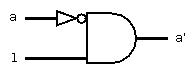
\includegraphics[scale=0.7]{hw2-1a}

		Using one gate with inputs $a$ and $1$, a second taking the output of the first gate and $b$, and a third taking the second output and $1$, the gate can be used to create a NAND gate, which is universal.

		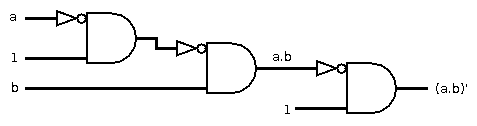
\includegraphics[scale=0.7]{hw2-1a2}

		\item[XOR] The XOR configuration cannot be made universal. As it is, it has the following truth table.

		\begin{tabular}{ c c c | c}
		$a$ & $\overline{a}$ & $b$ & $\overline{a} \oplus b$\\ \hline
		0 & 1 & 0 & 1\\
		0 & 1 & 1 & 0\\
		1 & 0 & 0 & 0\\
		1 & 0 & 1 & 1
		\end{tabular}

		This truth table is recognizeable as XNOR. A NOT gate can be made if either input is held at $0$.

		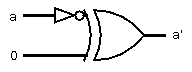
\includegraphics[scale=0.7]{hw2-1b} 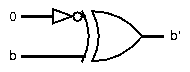
\includegraphics[scale=0.7]{hw2-1b2}

		Even with the addition of more NOT gates, the gate can only be made an XOR or XNOR.

		\begin{tabular}{ c c c c | c c c c}
		$a$ & $b$ & $\overline{a}$ & $\overline{b}$ & $\overline{a} \oplus b$ & $\overline{a} \oplus \overline{b}$ & $\overline{\overline{a}} \oplus b$ & $\overline{\overline{a} \oplus b}$\\ \hline
		0 & 0 & 1 & 1 & 1 & 0 & 0 & 0\\
		0 & 1 & 1 & 0 & 0 & 1 & 1 & 1\\
		1 & 0 & 0 & 1 & 0 & 1 & 1 & 1\\
		1 & 1 & 0 & 0 & 1 & 0 & 0 & 0
		\end{tabular}

		As such, this gate cannot be made universal.
	
	\end{itemize}
	
	\item[Question 2]\hspace{0pt}\\
		$f(a, b, c, d) = \Sigma (0, 1, 2, 3, 12, 13, 14, 15 )$\\
		\begin{Karnaugh}
			\minterms{0,1,2,3,12,13,14,15}
			\maxterms{4,5,6,7,8,9,10,11}
			\implicant{0}{2}{red}
			\implicant{12}{14}{purple}
		\end{Karnaugh}\\
		$f(a ,b , c, d) = \overline{a}.\overline{b} + a.b = \overline{a \oplus b}$\\\\

		$g(a, b, c, d) = \Sigma (0, 1, 2, 3, 4, 5, 6, 7, 8, 9, 10, 12, 13, 14, 15 )$\\
		\begin{Karnaugh}
			\minterms{0,1,2,3,4,5,6,7,8,9,10,12,13,14,15}
			\maxterms{11}
			\implicant{0}{14}{red}
			\implicant{2}{10}{purple}
			\implicant{0}{9}{blue}
		\end{Karnaugh}\\
		$g(a ,b , c, d) = \overline{a.\overline{b}} + \overline{c} + c.\overline{d} = \overline{a} + b + \overline{c} + c.\overline{d}$\\\\

		$h(a, b, c) = \Pi ( 0, 1, 2, 3 )$\\
		\begin{Karnaughvuit}
			\minterms{4,5,6,7}
			\maxterms{0,1,2,3}
			\implicant{4}{6}{red}
		\end{Karnaughvuit}\\
		$h(a, b, c) = a$\\\\

		$k(a, b, c, d) = \Pi (0, 1, 7, 8 )$\\
		\begin{Karnaugh}
			\minterms{2,3,4,5,6,9,10,11,12,13,14,15}
			\maxterms{0,1,7,8}
			\implicant{4}{13}{red}
			\implicant{13}{10}{purple}
			\implicant{2}{10}{blue}
			\implicant{3}{2}{green}
		\end{Karnaugh}\\
		$k(a ,b , c, d) = b.\overline{c} + a.(c + d) + c.\overline{d} + c.\overline{a}.\overline{b}\\
		= b.\overline{c} + a.c + a.d + c.(\overline{d} + \overline{a}.\overline{b})\\
		= a(c + d) + b.\overline{c} + c.(\overline{d} + \overline{a}.\overline{b})$

	\item[Question 3]\hspace{0pt}\\
	\begin{tabular}{c c c | c c c c c c c c}
	$a$ & $b$ & $c$ & majority voter\\ \hline
	0 & 0 & 0 & 0\\
	0 & 0 & 1 & 0\\
	0 & 1 & 0 & 0\\
	0 & 1 & 1 & 1\\
	1 & 0 & 0 & 0\\
	1 & 0 & 1 & 1\\
	1 & 1 & 0 & 1\\
	1 & 1 & 1 & 1 
	\end{tabular}\\\\
	Active-High:\\
	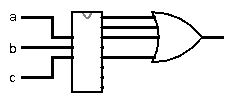
\includegraphics[scale=0.7]{hw2-3a}\\\\
	Active-Low with Active-Low Enable:\\
	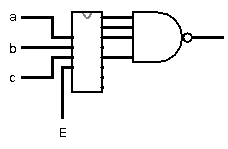
\includegraphics[scale=0.7]{hw2-3b}

	\item[Question 4]\hspace{0pt}\\

	\lstinputlisting[language=Python]{homework2.py}

	\begin{tabular}{ c c c c | c c c c c c c c }
	E & a & b & c & D7 & D6 & D5 & D4 & D3 & D2 & D1 & D0 \\\hline
	0 & 0 & 0 & 1 & 0 & 0 & 0 & 0 & 0 & 0 & 0 & 0 \\
	0 & 0 & 0 & 0 & 0 & 0 & 0 & 0 & 0 & 0 & 0 & 0 \\
	0 & 0 & 1 & 0 & 0 & 0 & 0 & 0 & 0 & 0 & 0 & 0 \\
	0 & 0 & 1 & 1 & 0 & 0 & 0 & 0 & 0 & 0 & 0 & 0 \\
	0 & 1 & 0 & 0 & 0 & 0 & 0 & 0 & 0 & 0 & 0 & 0 \\
	0 & 1 & 0 & 1 & 0 & 0 & 0 & 0 & 0 & 0 & 0 & 0 \\
	0 & 1 & 1 & 0 & 0 & 0 & 0 & 0 & 0 & 0 & 0 & 0 \\
	0 & 1 & 1 & 1 & 0 & 0 & 0 & 0 & 0 & 0 & 0 & 0 \\
	1 & 0 & 0 & 0 & 0 & 0 & 0 & 0 & 0 & 0 & 0 & 1 \\
	1 & 0 & 0 & 1 & 0 & 0 & 0 & 0 & 0 & 0 & 1 & 0 \\
	1 & 0 & 1 & 0 & 0 & 0 & 0 & 0 & 0 & 1 & 0 & 0 \\
	1 & 0 & 1 & 1 & 0 & 0 & 0 & 0 & 1 & 0 & 0 & 0 \\
	1 & 1 & 0 & 0 & 0 & 0 & 0 & 1 & 0 & 0 & 0 & 0 \\
	1 & 1 & 0 & 1 & 0 & 0 & 1 & 0 & 0 & 0 & 0 & 0 \\
	1 & 1 & 1 & 0 & 0 & 1 & 0 & 0 & 0 & 0 & 0 & 0 \\
	1 & 1 & 1 & 1 & 1 & 0 & 0 & 0 & 0 & 0 & 0 & 0 \\
	\end{tabular}

\end{itemize}

\end{document}